% reset section counter
%\setcounter{section}{0}

%\metadata{lecture ID}{Your names}{date}
\metadata{13}{Justin Young and Josh Cho}{November 1, 2021}

\sec{The Neural Tangent Kernel (NTK) Approach}

In the previous sections, we studied non-convex optimization problems in which all local minima are global. Here we consider an objective for which we can identify particular regions of the input space in which all local minima are also global minima. \tnote{a bit better transition and positioning, e.g., specify that this only works for certain cases; also add some literature}

\tnotelong{Tengyu should  double check this later}

To be more formal, we take an appropriate parameter initialization $\theta^0$ such that in a neighborhood around it, which we denote by $B(\theta^0)$, the loss function is convex and its global minimum is attained. Figure \ref{lec13:fig:NTKapproach} depicts a function and region for which this condition holds. 

\begin{figure}[ht]
    \centering
    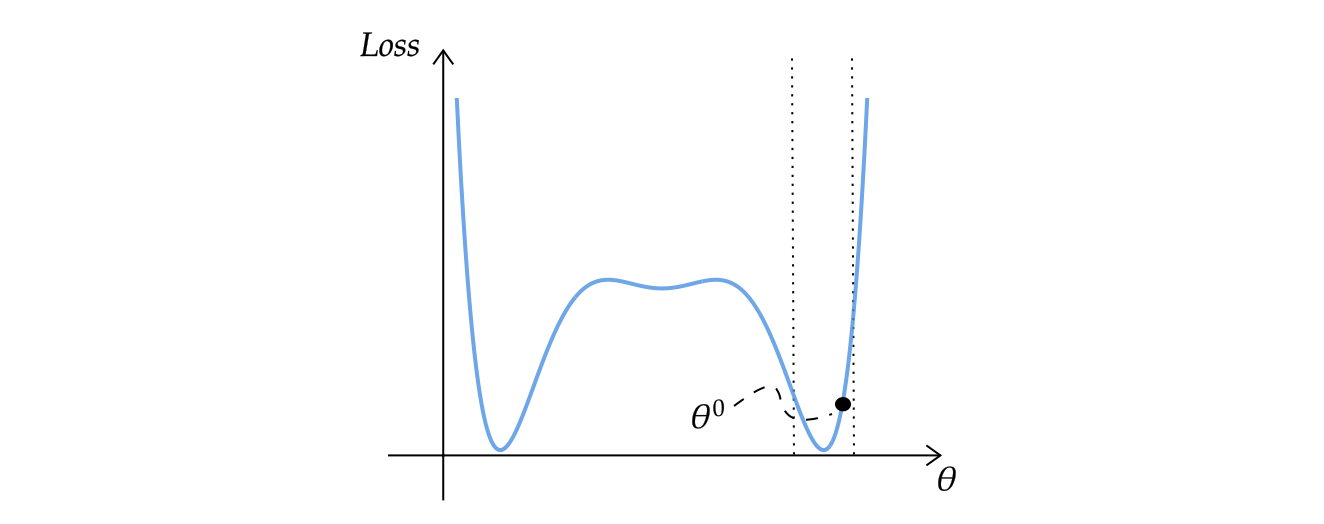
\includegraphics[scale=0.5]{figures/ntk_initialization.png}
    \caption{Training loss around an initialized $\theta^0$. The dotted lines indicate $B(\theta^0)$, a region where the loss is convex, and where a global minimum exists.
    	\tnote{(a) have two equally good global min. (b) make the global min have y-value zero or near zero. }
    }
    \label{lec13:fig:NTKapproach}
\end{figure}


Given a nonlinear $f_\theta(x)$, we examine the Taylor expansion at $\theta^0$: 
\begin{align} 
    f_\theta(x) = \underbrace{f_{\theta^0}(x) + \langle \nabla_\theta f_{\theta^0}(x),\theta-\theta^0 \rangle}_{\defeq g_\theta(x)} + \text{ higher order terms}
\end{align} 

Note that $g_\theta(x)$ is an affine function in $\theta$, as $f_{\theta^0}(x)$ is a constant for fixed $x,\theta^0$. Similarly, defining $\Delta \theta = \theta-\theta^0$, we can say that $g_\theta(x)$ is linear in $\Delta \theta$. For convenience, we will sometimes choose $\theta^0$ such that $f_{\theta^0}(x) = 0$ for all $x$. It is easy to see why such an initialization exists. Consider splitting a two-layer neural network $f_{\theta}(x)$ with width $2m$ into two halves, each with $m$ neurons; the outputs of these two networks are then given by $\sum_{i=1}^m a_i \sigma (w_i^\top x)$ and $\sum_{i=1}^m -a_i \sigma (w_i^\top x)$, respectively. Here, $w_i$ can be randomly chosen so long as $W_i$ is the same in both halves, and $a_i$ can be randomly chosen as long as the other half is initialized with $-a_i$. Summing these two networks together yields $f_{\theta^0}(x) \equiv 0$ for all $x$.

Letting 
\begin{align}
    y' &= y- f_{\theta^0}(x) \\
    &= \inprod{\nabla_\theta f_{\theta^0}(x), \Delta \theta},
\end{align}
we observe that $\Delta \theta$ depends upon the parameter we evaluate the network at, while $\nabla_\theta f_{\theta^0}(x)$ can be thought of as a feature map since it is a fixed function of $x$ (given the architecture and $\theta^0$) that does not depend on $\theta$ whatsoever. We thus let $\phi(x) \triangleq \nabla_\theta f_{\theta^0}(x)$, which motivates the following definition: 

\begin{definition}[Neural Tangent Kernel]
For simplicity, we assume $f_{\theta^0}(x)=0$ so that $y=y'$. The \textit{neural tangent kernel} $K$ is given by  
\begin{align} 
    K(x,x') &= \inprod{\phi(x), \phi(x')} \\
    &= \inprod{\nabla_\theta f_{\theta^0}(x), \nabla_\theta f_{\theta^0}(x')}.
\end{align} 
\end{definition}
Here, the feature $\nabla_\theta f_{\theta^0}(x)$ is precisely the gradient of the neural network. This is where the ``tangent'' in Neural Tangent Kernel comes from. 

Instead of $f_\theta(x)$, suppose we use the approximation $g_\theta(x)$, which we recall is linear in $\theta$. The kernel method gives a linear model on top of features. When $\theta \approx {\theta^0}$, given a convex loss function $\ell$, we have 
\begin{align} 
    \underbrace{\ell (f_\theta(x),y)}_{\substack{\text{not} \\ \text{necessarily} \\ \text{convex}}} \approx \underbrace{\ell(g_\theta(x),y)}_{\text{convex}}.
\end{align} 
Convexity of the RHS follows from the fact that a convex function, $\ell$, composed with a linear function, $g_\theta$, is still convex. 

A natural question to ask is: how valid is this approximation? We devote the rest of this chapter to answering this question. First, we define the empirical loss: 
\begin{align}
    \hat{L}(f_\theta) & = \frac{1}{n}\sum_{i=1}^n \ell \left( f_\theta\big( x^{(i)} \big) , y^{(i)} \right) \\ 
    \hat{L}(g_\theta) & = \frac{1}{n}\sum_{i=1}^n \ell \left( g_\theta\big( x^{(i)} \big) , y^{(i)} \right).
\end{align} 
The key idea is that the Taylor approximation works for certain cases. We defer a more complete enumeration of these cases to a later section of this monograph. For now, we claim that this Taylor expansion is valid for the following situation\tnote{rephrase a bit? maybe "Here we outline the high-level approach to validate and use the Taylor expansion.."}. 
 We assume \tnote{reword -- we will show instead of assume} that there exists a neighborhood around $\theta^0$ called $B(\theta^0)$, such that we have the following:
\begin{enumerate}
    \item Accurate approximation: $f_\theta(x) \approx g_\theta(x)$, and $\hat{L}(f_\theta) \approx \hat{L}(g_\theta)$ for all $\theta \in B(\theta^0)$.
    \item It suffices to optimize in $B(\theta^0)$: There exists an approximate global minimum $\hat{\theta} \in B(\theta^0)$, so $\hat{L}(g_{\hat{\theta}}) \approx 0$. This is the lowest possible loss (because the loss is nonnegative), which implies we are close to the global minimum. Because of 1, this implies that $\hat{L}(f_{\hat{\theta}}) \approx 0$ as well.
    \item Optimizing $\hat{L} (f_\theta)$ is similar to optimizing $\hat{L}(g_\theta)$ and does not leave $B(\theta^0)$, i.e. everything is confined to this region. Intuitively, this last point to some extent is ``implied" by (1) and (2), but this claim still requires a formal proof. 
\end{enumerate}
Note (1), (2), and (3) can all be true in various settings. In particular, to attain all three, we will require: 
\begin{enumerate}[label=\alph*]
    \item[(a)] Overparametrization and/or a particular scaling of the initialized $\theta^0$. 
    \item[(b)] Small (or even zero) stochasticity, so $\theta$ never leaves $B(\theta^0)$. This condition is guaranteed by a small learning rate or full-batch gradient descent. 
\end{enumerate} 
Despite the limitations of the requirements of (a) and (b), the existence of such a region is still surprising. Given the loss landscape which could potentially be highly non-convex, it is striking to find a neighborhood where the loss function is convex (e.g. quadratic) with a global minimum. This suggests there is some flexibility in the loss landscape.  

To begin our formal discussion, we  start by providing tools for proving (1) and (2). Let 
\begin{align}
    \phi^{(i)} = \phi(x\sp{i}) = \nabla_\theta f_{\theta^0}( x\sp{i}) \in \R^p
\end{align}
and 
\begin{align}
    \Phi = \begin{bmatrix} {\phi\sp{1}}^\top \\ \vdots \\ {\phi\sp{n}}^\top \end{bmatrix} \in \R^{n \times p}
\end{align}
where $p$ is the number of parameters. Taking the quadratic loss, we have
\begin{align}
    \hat{L}(g_\theta) = \frac{1}{n}\sum_{i=1}^n \left( y\sp{i} - \phi\l(x\sp{i} \r)^\top \Delta \theta \right)^2 = \frac{1}{n} \norm{\vec{y} - \Phi \cdot \Delta \theta}_2^2
\end{align} 
where $\vec{y} = \l[ y\sp{1}, \cdots, y\sp{n} \r]^\top \in \R^n$. Note that this looks a lot like linear regression, where $\Phi$ and $\Delta \theta$ are the analogues of the design matrix and parameter, respectively. We further assume that $y^{(i)} = O(1)$ and $\norm{y}_2 = O(\sqrt{n})$. Now, we can prove a lemma that addresses the second of the three conditions we described above, i.e. that it is sufficient to optimize in some small ball around $\theta^0$.

\begin{lemma}[for (2)] 
    Suppose we are in the setting where $p \geq n$, $\textup{rank}(\Phi) = n$, and $\sigma_{\min}(\Phi) = \sigma > 0$. Then, letting $\Delta \hat{\theta}$ denote the minimum norm solution, i.e. the nearest global minimum, of $\vec{y} = \Phi \Delta \theta$, we have 
    \begin{align} 
        \norm{\Delta \hat{\theta}}_2 \leq O(\sqrt{n} / \sigma)
    \end{align} 
\end{lemma}
\begin{remark} \label{lec13:rmk:intuitiononlemma} 
    The meaning of the bound on $\Delta \hat{\theta}$ becomes clear if we consider the ball given by 
    \begin{align}
        B_{\theta^0} = \{ \theta = \theta^0 + \Delta \theta: \norm{\Delta \theta}_2 \leq O(\sqrt{n}/\sigma )\}.
    \end{align} 
    In particular, notice that $B_{\theta^0}$ contains a global minimum, so this lemma characterizes how large the ball must be to contain a global minimum. 
    \end{remark} 
\begin{remark}
	We also note that the condition $\textup{rank}(\Phi) = n$ and $\sigma > 0$ can be thought of as a ``finite-sample expressivity'' condition, saying that the features $\Phi$ are expressive enough so that there exists a linear model on top of these features that perfectly fit the data. The condition $\textup{rank}(\Phi) = n$ requires $p \ge n$---so we need some amount of over-parameterization to apply these analysis. 
\end{remark}
\tnote{replace dagger by $+$ to be consistent with wikipedia (I think this applies to some previous lectures which I commented on as well)}
\begin{proof}
    Letting $\Phi^\dagger$ denote the Moore-Penrose pseudoinverse of $\Phi$, note that $\Delta \hat{\theta} = \Phi^\dagger \boldsymbol{y}$, and $\norm{\Phi^\dagger} _{\text{op}} = \frac{1}{\sigma_{\min} (\Phi)} = \frac{1}{\sigma}$.  A simple argument shows 
    \begin{align}
        \norm{\Delta \hat{\theta}}_2 &\leq \norm{\Phi^\dagger}_{\text{op}} \cdot \norm{\vec{y}}_2 \\
        &\leq O\left( \frac{1}{\sigma}\cdot \sqrt{n} \right),
    \end{align} 
    where the last inequality follows from the assumption that $\norm{\vec{y}}_2 \leq O(\sqrt{n})$. 
\end{proof}
Next, we prove a lemma that addresses the first of the three steps we described above.
\begin{lemma}[for (1)] 
    \label{lec13:lma:accurate_approximation}
    Suppose $\nabla_\theta f_\theta(x)$ is $\beta$-Lipschitz in $\theta$, i.e. for every $x$, and $\theta, \theta'$, we have 
    \begin{align}
        \norm{\nabla_\theta f_{\theta} (x) - \nabla_{\theta} f_{\theta'}(x)}_2 \leq \beta \cdot \norm{ \theta - \theta'}_2.
    \end{align} 
    Then, 
    \begin{align} 
        \left| f_\theta(x) - g_\theta(x) \right| \leq O \left( \beta \norm{\Delta \theta}_2^2 \right|.
    \end{align}  
    \tnote{typo above}
    If we further restrict our choice of $\theta$ using $B_{\theta^0}$ as defined in Remark~\ref{lec13:rmk:intuitiononlemma}, we obtain that
    \begin{align} 
        | f_\theta(x) - g_\theta(x) | \leq O \left( \frac{\beta n }{\sigma^2 }\right), \quad \forall \theta \in B_{\theta^0}. \label{lec13:eqn:lemma1bound} 
    \end{align} 
\end{lemma}
\begin{proof}
    The proof comes from the following fact:  if $h(\theta)$ is such that $\nabla h(\theta)$ is $\beta$-Lipschitz (which if differentiable is equivalent to $\norm{\nabla^2 h(\theta)}_{\text{op}} \leq \beta$), then
    \begin{align}
        \bigg| \underbrace{h(\theta)}_{f_\theta(x)}  \underbrace{-h(\theta^0) - \inprod{\nabla h(\theta^0), \theta-\theta^0}}_{-g_\theta(x)}\bigg| \leq O\left( \beta \norm{\theta-\theta^0}_2^2 \right).
    \end{align} 
    \tnotelong{add a lemma in the toolbox section about this}
    As shown above, the proof is as simple as plugging in $f_\theta(x) = h(\theta)$ and $g_\theta(x)=h(\theta^0) + \inprod{\nabla h(\theta^0), \Delta \theta}$. 
\end{proof}

\begin{remark}
The lemma above bounds the approximation error. Intuitively, as you move farther away from $\theta^0$, the Taylor approximation gets worse; the approximation error is bounded above by a second order $\Delta \theta$ term.
\end{remark}

\begin{remark}
Note that if $f_\theta$ involves a $\text{relu}$ function, then $\nabla f_\theta$ is not continuous everywhere. This requires a technical fix outside the scope of our discussion.\footnote{A $\text{relu}$ function is continuous almost everywhere, so we can make some minor fixes and still use some modified notion of Lipschitzness to derive an upper bound.} \tnote{Tengyu will add a reference here}
\end{remark}

\subsec{Two examples of the NTK regime}
By \eqref{lec13:eqn:lemma1bound}, we have now established a bound on our approximation error, but we have yet to analyze how good it is, as $\beta n /\sigma^2$ is neither obviously either big nor small. An important fact to notice is that $\beta/\sigma^2$ is not scaling invariant, so we can play with the scaling in order to drive this term to $0$. In particular, there are two notable cases (with specific parameterization, initialization, etc) where $\beta/\sigma^2 \to 0$. In the literature, such situation is often referred to as the NTK regime or the lazy training regime~\cite{chizat2018note}. 
\begin{enumerate}
    \item  \textbf{Reparametrize with a scalar} \cite{chizat2018note}. Let $f_\theta(x) = \alpha \cdot \bar{f}_\theta(x)$ where $\bar{f}_\theta(x)$ is an arbitrary neural net with fixed width and depth. We only vary $\alpha$, i.e. the scaling, and we see how the crucial quantity $\beta/\sigma^2$ changes accordingly. Fix an initial $\theta^0$, and let 
    \begin{align}
        \bar{\sigma} = \sigma_{\min}\left( \begin{bmatrix}  \nabla_\theta \bar{f}_{\theta^0} \big( x^{(i)} \big)^\top \\ \vdots \\ \nabla_\theta \bar{f}_{\theta^0} \big(x^{(i)} \big)^\top \end{bmatrix}\right).
    \end{align} 
    Furthermore, let $\bar{\beta}$ be the Lipschitz parameter of $\nabla_\theta \bar{f}_\theta(x)$ in $\theta$. A simple chain-rule gradient argument shows that scaling $\bar{f}_{\theta}$ by $\alpha$ also scales $\sigma$ and $\beta$ accordingly, i.e. $\sigma = \alpha \bar{\sigma}$, and $\beta = \alpha \bar{\beta}$. Some straightforward algebra yields 
    \begin{align} 
        \frac{\beta}{\sigma^2}= \frac{\bar{\beta}}{\bar{\sigma}^2} \cdot \frac{1}{\alpha} \to 0 \quad \text{as} \quad \alpha \to \infty.
    \end{align}
    Once $\alpha$ becomes big enough, then by Lemma~\ref{lec13:lma:accurate_approximation}, the approximation $|f_\theta(x) - g_\theta(x)| \leq O\left( \beta n / \sigma^2 \right)$ becomes very good.  
    \begin{remark}
    Note that this scaling does not scale the loss. Intuitively, while the function $f_\theta$ becomes sharper and non-smooth as $\alpha$ grows big (leading to higher approximation error), we note that we only need to travel a little bit away from $\theta^0$ given the $\beta$-Lipschitz constraint on the gradient of $f_{\theta}$. In particular, the neighborhood around $\theta^0$ shrinks faster than the approximation error grows.  
    \end{remark}
    \item \textbf{Overparametrization (with specific initialization)}. Early papers on the NTK take this approach. Consider a  two-layer network with $m$ neurons. 
    \begin{align}
        \hat{y} = \frac{1}{\sqrt{m}} \sum_{i=1}^m a_i \sigma(w_i^\top x )
    \end{align} 
    The scaling $1/\sqrt{m}$ will be for convenience, as we see momentarily. We make the following assumptions regarding the network and its inputs.
    \begin{align}
        W &= \begin{bmatrix} w_1^\top \\ \vdots \\ w_m^\top \end{bmatrix} \in \R^{m \times d} \\
        \sigma &\text{ is $1$-Lipschitz and twice-differentiable} \\
        a_i &\sim \{\pm 1\} \quad &\text{(not optimized)} \\
        w_i^0 &\sim \cN(0, I_d) \\
        \norm{x}_2 &= \Theta(1) \\
        \theta &= \text{vec}(W) \in \R^{dm} \quad &\text{(vectorized $W$)}
    \end{align} 
    We will assume $m \to \infty$, and in particular, for fixed $n,d$, $m = \textsf{poly}(n,d)$.
    
    Why do we use the $1/\sqrt{m}$ scaling? Note that $\sigma\big({w_i^0}^\top x\big) \approx 1$ because $\norm{x}_2 = \Theta(1)$ and $w_i^0$ is drawn from a spherical Gaussian. Thus, as some $a_i$ are positive and others are negative, $\left|\sum_{i=1}^m a_i \sigma \big({w_i^0}^\top x\big) \right| = \Theta \left( \sqrt{m} \right)$, and finally $f_{\theta^0} (x) = \Theta(1)$. 
    
    Now we analyze $\sigma$ and $\beta$. We let
    \begin{align}
        \sigma = \sigma_{\min} (\Phi) = \sqrt{\sigma_{\min} \left( \Phi \Phi^\top \right)}
    \end{align}
    where 
    \begin{align}
        \left( \Phi \Phi^\top \right)_{ij} = \inprod{\nabla_\theta f_{\theta^0} \big(x^{(i)} \big) , \nabla_\theta f_{\theta^0} \big(x^{(j)} \big)} \label{lec13:eqn:phifeature} 
    \end{align} 
    Note that the gradient with respect to $w_i$ is given by 
    \begin{align}  
        \frac{\partial f_\theta(x) }{\partial w_i} = \frac{1}{\sqrt{m}} \sigma'(w_i^\top x ) \cdot x 
    \end{align} 
    Now observe that
    \begin{align}
        \norm{\nabla f_\theta(x)}_2^2 & = \frac{1}{m}\sum_{i=1}^m \norm{\sigma'\big({w_i}^\top x \big) \cdot x }_2^2 \\ 
        & = \frac{1}{m}\norm{x}_2^2 \cdot \sum_{i=1}^m \left( \sigma' \big({w_i}^\top x \big) \right)^2 \\ 
        &\to \Exp_{w \sim \cN(0,I_d)} \left[ \sigma' \big( w^\top x \big)^2 \right] \cdot \norm{x}_2^2 \quad \text{as} \quad m\to\infty \\ 
        &= O(1) &\text{(not depending on $m$)}
    \end{align} 
    where the penultimate line follows from the law of large numbers, as $\frac{1}{m} \sum_{i=1}^m \left( \sigma'(w_i^\top x ) \right)^2$ can be interpreted as a mean. 
    
    Note that $\norm{\nabla_\theta f_{\theta^0} (x)}_2$ does not depend on $m$, so the inner product in \eqref{lec13:eqn:phifeature} also does not depend on $m$ either. As above, we can show 
    \begin{align} 
        \inprod{\nabla_\theta f_{\theta^0} (x), \nabla_\theta f_{\theta^0} (x')} & = \frac{1}{m}\inprod{ x,x'} \sum_{i=1}^m \sigma'(w^\top x) \sigma'(w^\top x')  \\ 
        & \to \Exp_{w \sim \cN(0,I_d)} \left[ \sigma'(w^\top x) \sigma'(w^\top x') \right] \inprod{ x, x'} \label{lec13:eqn:kernelcalc} 
    \end{align}
    
    \eqref{lec13:eqn:kernelcalc} implies that as $m \to \infty$, $\Phi \Phi^\top$ converges to a constant matrix denoted by 
    \begin{align}
        K^\infty = \lim_{m \to \infty} \Phi\Phi^\top 
    \end{align}
    This is precisely the NTK with $m=\infty$. 
    
    Though we omit the proof of this claim, it can be shown that $K^\infty$ is full rank. Then, let \begin{align}
        \sigma_{\min} \triangleq \sigma_{\min} (K^\infty) > 0.
    \end{align}
    We can show that 
    \begin{align}
        \sigma = \sigma_{\min} \left( \Phi \Phi^\top \right) > \frac{1}{2}\sigma_{\min} 
    \end{align} 
    Intuitively, $\Phi \Phi^\top \to K^\infty$, so the spectrum of the matrix should also converge. Thus, in some sense, we have shown that $\sigma$ is constant in the limit. 
    
    Now what about $\beta$? If we can show $\beta \to 0$ as $m \to \infty$, we are done. We begin by analyzing this key expression:  
    \begin{align}
        \nabla_\theta f_\theta(x) - \nabla_\theta f_{\theta'} (x) = \left[ \frac{1}{\sqrt{m}} \left( \sigma' \big( w_i^\top x \big) - \sigma' \big({w_i'}^\top x \big) \right) \cdot x \right]_{i=1}^m \label{lec13:eqn:lipschitzmatrix}
    \end{align}
    Note that \eqref{lec13:eqn:lipschitzmatrix} above consists of matrices, as $\theta$ is a vectorized matrix. Then,
    \begin{align}
        \norm{\nabla_\theta f_\theta(x) - \nabla_\theta f_{\theta'}(x)}_2^2 & = \frac{1}{m}\sum_{i=1}^m \norm{x}_2^2 \left( \sigma' \big(w_i^\top x \big) - \sigma' \big({w_i}'^\top x \big) \right)^2  \\ 
        & \leq O \left( \frac{1}{m}\sum_{i=1}^m \norm{ x}_2^2 \big( w_i^\top x - {w_i'}^\top x \big)^2 \right) \\ 
        & =  O \left( \frac{1}{m}\sum_{i=1}^m \norm{ w_i - w_i'}_2^2 \right) \\ 
        & = O \left(\frac{1}{m} \norm{ \theta - \theta' }_2^2 \right)
    \end{align} 
    The first line follows from the fact that $\frac{1}{\sqrt{m}} \left( \sigma' \big( w_i^\top x \big) - \sigma' \big({w_i'}^\top x \big) \right)$ is a scalar. The second line uses the assumption that $\sigma'$ is $O(1)$-Lipschitz. The third line uses Cauchy-Schwarz and the fact that $\norm{x}_2^2 \approx 1$. Taking the square root, we have that
    \begin{align} 
        \norm{\nabla_\theta f_\theta(x) - \nabla_\theta f_{\theta'}(x)}_2 \lesssim \frac{1}{\sqrt{m} } \norm{ \theta -\theta' }_2
    \end{align} 
    Thus, the Lipschitz parameter is $\beta = O(1/\sqrt{m})$. Thus, our key quantity $\beta/\sigma^2$ goes to $0$ as $m$ grows. Namely,
    \begin{align} 
        \frac{\beta}{\sigma^2} \approx \frac{1}{\sqrt{m} }\cdot \frac{1}{\sigma_{\min}^2} \to 0 \quad \text{as} \quad m\to\infty.
    \end{align} 
    Recall here that $\sigma_{\min}$ does not depend on $m$. Concretely, this result tells us that our function becomes more smooth (the gradient has a smaller Lipschitz constant) as we add more neurons. 
\end{enumerate}

\subsec{Optimizing $\hat{L}(g_\theta)$ vs. $\hat{L}(f_\theta)$}
We now discuss how to establish the last of the three conditions under which we claimed a Taylor approximation is reasonable. We need to show that  optimizing $\hat{L} (f_\theta)$ is similar to optimizing $\hat{L}(g_\theta)$. To do so, we require two steps:
\begin{enumerate}[label=\alph*]
    \item[(A)] Analyze optimization of $\hat{L}(g_\theta)$.
    \item[(B)] Analyze optimization of $\hat{L}(f_\theta)$ by re-using the proof in (A).
\end{enumerate}
There are two approaches in the literature for (A), which implies that there exist two approaches for (B) as well. 
\begin{enumerate}
    \item[(i)] We leverage the strong convexity of $\hat{L} (g_\theta)$, and then show an exponential convergence rate.\footnote{Recall that a differentiable function $f$ is strongly convex if 
    \begin{align} 
        f(y) \geq f(x) + \nabla f(x)^\top (y-x) + \frac{\mu}{2} \norm{y-x}_2^2
    \end{align} for some $\mu>0$ and all $x,y$.} 
    \item[(ii)] Instead of strong convexity, we use smoothness of $f_\theta$ (i.e. bounded second derivative). 
\end{enumerate}
We will only discuss the first of these two methods in this monograph.

\begin{remark} 
Suppose at any $\theta^t$, we take the Taylor expansion of $g_\theta$ at $\theta^t$ so 
\begin{align} 
    g_\theta^t(x) = g_{\theta^t} (x) + \inprod{ \nabla f_{\theta^t} (x),\theta-\theta^t } 
\end{align} 
Consider the gradient we are interested in taking: $\nabla \hat{L} ( f_{\theta^t})$. Notice that: \begin{align} 
    \nabla \hat{L} ( f_{\theta^t}) = \nabla \hat{L} ( g_{\theta^t}^t)
\end{align} 
This is really saying that $f_\theta$ and $g_\theta^t$ agree up to first-order at $\theta^t$. This implies that $L(f_\theta)$ and $L(g_\theta^t)$ also agree up to the first-order at $\theta^t$. This means that $T$ steps of gradient descent on $\hat{L}(f_\theta)$ is the same as performing online gradient descent\footnote{See Chapter~\ref{chap:OL}.} on a sequence of changing objectives $L(g_\theta^0), \ldots, L(g_\theta^T)$.
\end{remark} 